\documentclass[10pt,a4paper]{article}

% include stuff
\usepackage[utf8]{inputenc}
\usepackage[obeyDraft]{todonotes}
\usepackage{hyperref}
\usepackage{amssymb}
\usepackage{longtable}
\usepackage{multirow}
\usepackage[T1]{fontenc}
\usepackage{xkeyval}
% TODO
%\define\choicekey*{fam}{method}[]{call-1,call-2,pileup,rt-arrest,lrt-arrest}{%
%    
%}

\newcommand{\callone}{call-1}
\newcommand{\calltwo}{call-2}
\newcommand{\pileup}{pileup}
\newcommand{\rtarrest}{rt-arrest}
\newcommand{\lrtarrest}{lrt-arrest}

\newcommand{\clioption}[3]{%
    \begin{tabular}{p{.3\textwidth}p{.7\textwidth}}
        #1 & #2 \\
           & \hfill #3 \\
    \end{tabular}
}

% document relatedf
\title{JACUSA2 manual}
\author{Michael Piechotta \\ michael.piechotta@gmail.com}
\date{29th, September, 2019} 

% TODO
% * structure CLI options
% * add command for formatting CLI options
% * add command to depict what method supports CLI opiton 
% * add command to depict what method supports what is required and what is optional
% --------------------------------------------------------------------------------------------------
\begin{document}
% --------------------------------------------------------------------------------------------------
\maketitle 
\tableofcontents
\listoftodos
% --------------------------------------------------------------------------------------------------
\section{Introduction}
JAVA framework for accurate Variant assessment (JACUSA2) is a one-stop solution to detect single
nucleotide variants (SNVs) and reverse transcriptase induced arrest events (RTAs) in Next-generation 
sequencing (NGS) samples.

\url{https://github.com/dieterich-lab/JACUSA2/}{JACUSA2} direct successor of 
\url{https://github.com/dieterich-lab/JACUSA/}{JACUSA1} --- JACUSA1 is hereby deprecated and won't be 
continued. All methods (call-1, call-2, and pileup) from JACUSA1 are available in JACUSA2. 
The new release of JACUSA2 features great performance enhancements (~3 faster) for existing methods and adds 
new methods (rt-arrest and lrt-arrest) that allow to identify read arrest events. 

\begin{figure}[t]
	\centering
	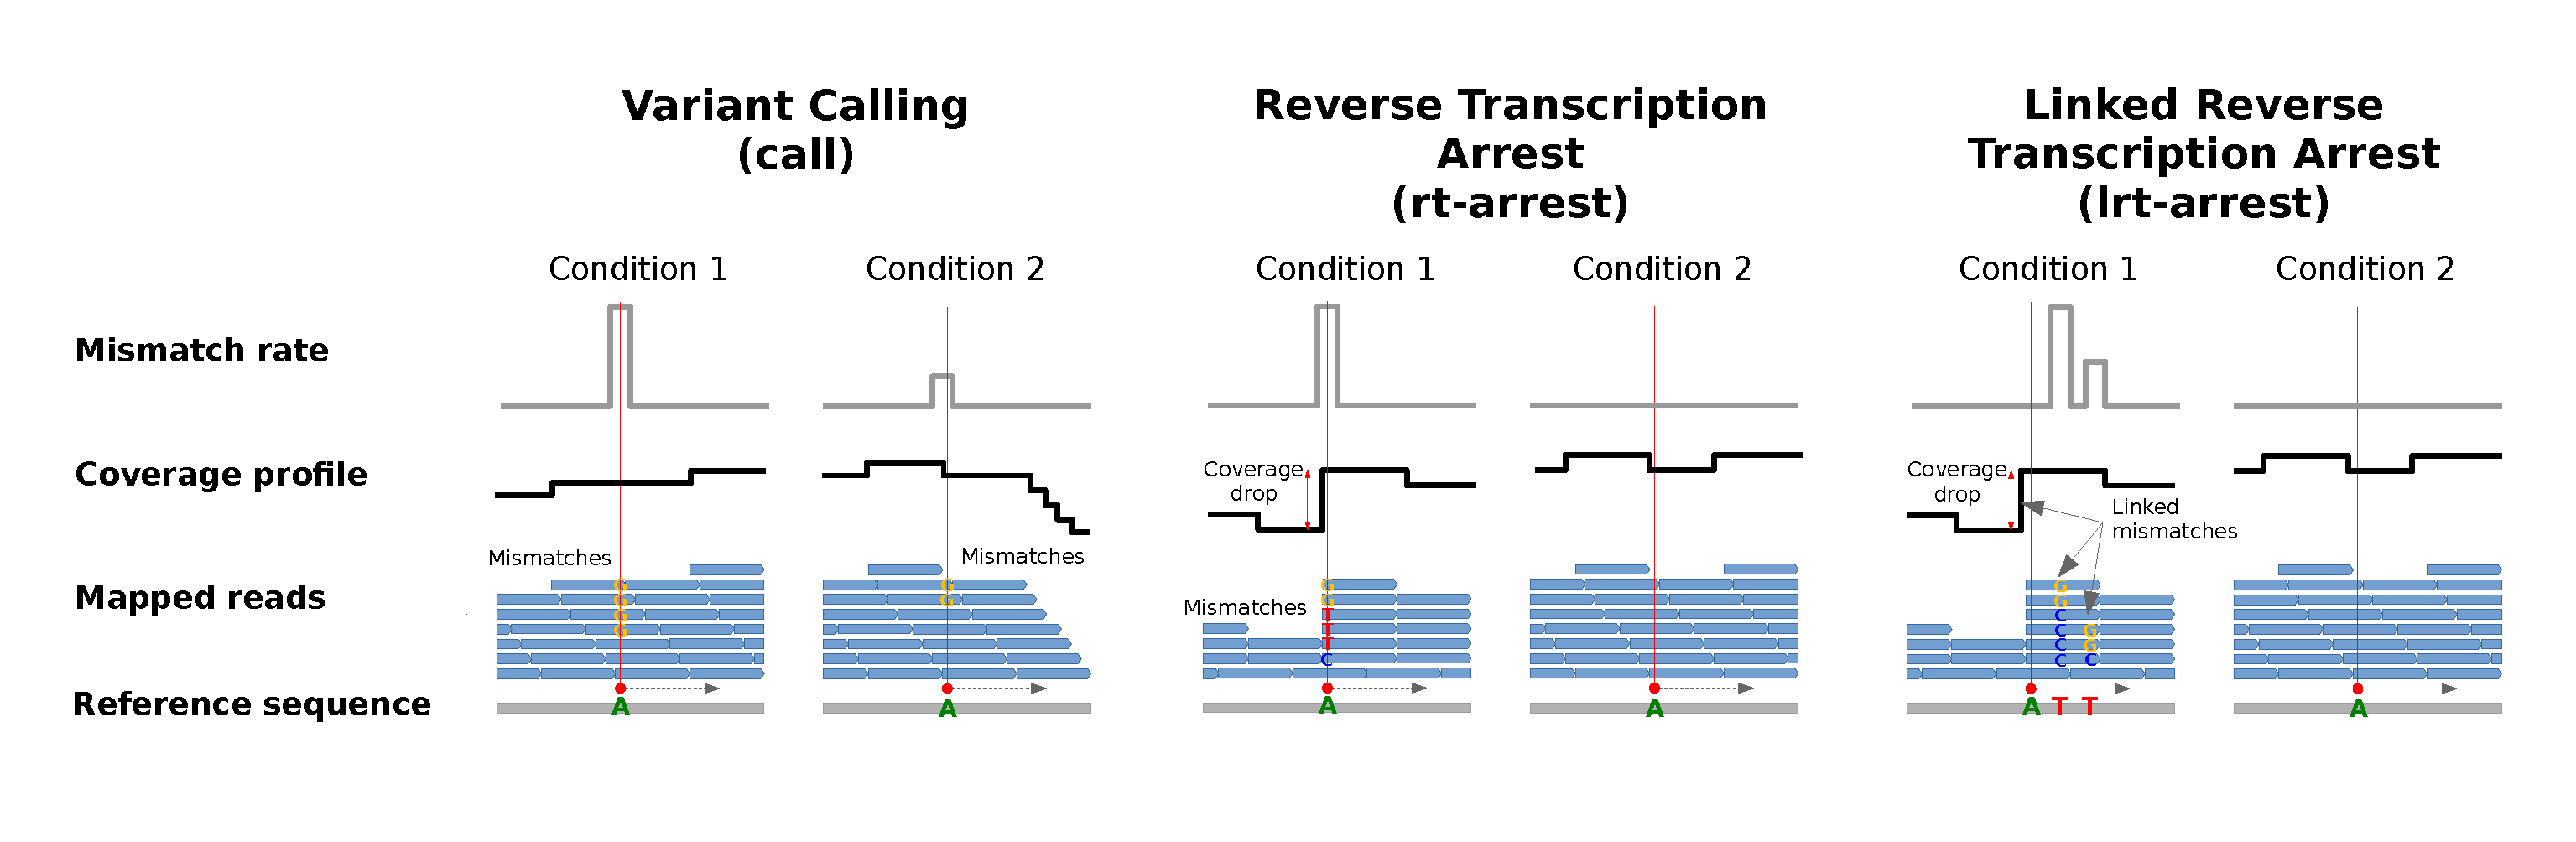
\includegraphics[width=\textwidth]{figures/poster_jacusa_methods.pdf}
\end{figure}

``rt-arrest'' allows to identify read arrest events by means of modelling read through counts and 
read arrest counts with a Beta-Binomial distribution. Likelihood ratio test that compares counts from two conditions
allows to identify statistically significants different sites. ``lrt-arrest'' is a combination of variant and arrest event detection.

Some of the artefact filters in JACUSA have been moved to the R helper package called JACUSA2helper (TODO link).
A new artefact filter has been added to JACUSA2 that allows to mark or filter candidate variants or arrest events 
by means of a file that contains sites to be excluded.

An other new feature in JACUSA2, is optional data that can be added to the output for some methods. 
Such optional data are INDEL count and differential statistics and read substitutions.
A user defined base substitution can be used to partition read in two sets: all reads and reads 
containing the user specified base substitution.   
 
JACUSA2 employs a window-based approach to traverse provided BAM files featuring highly parallel 
processing and utilizing the new \url{https://github.com/samtools/htsjdk}{htsjdk} framework.
% --------------------------------------------------------------------------------------------------
\subsection{Variant calling}
Robust identification of variants has proven to be a daunting task due to artefacts specific 
for NGS-data and employed mapping strategies. 
We implement various feature filters that reduce the number of false positives. 

JACUSA2 has been extensively evaluated and optimized to identify RNA editing sites in RNA-DNA and
RNA-RNA sequencing samples. Checkout the original publication of JACUSA1 \cite{Piechotta2017}.
% --------------------------------------------------------------------------------------------------
\subsection{Reverse transcriptase arrest events}
Reverse transcriptase arrest events can be induced during library preparation. 
They are identified by shorter than expected read length due to premature termination during first 
strand synthesis. Per site a vector of read through and read arrest can be calculated and compared 
between conditions. Read through and read arrest events are modelled by the Beta-Binomial distribution.
% --------------------------------------------------------------------------------------------------
\section{Download}
The latest version of JACUSA2 can be obtained from \url{https://github.com/dieterich-lab/JACUSA2/}{JACUSA2}.
Got to releases and pick the lastest release, currently: 
\url{https://github.com/dieterich-lab/JACUSA2/releases/download/2.0.0-RC12/JACUSA_v2.0.0-RC12.jar}{JACUSA2 2.0.0 RC12} 
% --------------------------------------------------------------------------------------------------
\subsection{Installation and requirements}
JACUSA2 does not need any configuration but needs a correctly configured Java environment.
We developed and tested JACUSA2 with Java v1.8. If you encounter any Java related problems please
consider to change to Java v1.8.
% --------------------------------------------------------------------------------------------------
\subsection{Migrating from JACUSA1 to JACUSA2}
There are several important changes to the command line interface:
\begin{itemize}
  \item ONLY single dash ``-'' options, e.g.: ``-c 10''. ALL two dash options ``--option [\ldots]'' have been removed.
  \item Use ``\textbf{-}filterNH'' and ``\textbf{-}filterNM'' instread of ``--filterNH''. 
	\item CLI format to provide library type has changed: JACUSA1: ``-P Lib1,Lib2'', JACUSA2: ``-P1 Lib1 -P2 Lib2''.
\end{itemize}
A new feature of JACUSA2 is a \#\#'' prefixed header line to the default output file format that 
contains command line options and used JACUSA2 version. The general layout of the default output has not changed.
% --------------------------------------------------------------------------------------------------
\subsection{Sample \textit{in silico} data}
\subsubsection{Variant calling}
You can choose between different setups and species where the later greatly influences the data size 
and running time to detect variants. The gDNA VS cDNA represents the typical data setup that is 
encountered in detection of RNA editing sites via comparing genomic and transcriptomic sequencing reads. 
In this setup, variants have been only imputed to the cDNA BAM file. The cDNA VS cDNA data setup can be interpreted as
representing allele specific expression of single variants or differential RNA editing. In this
setup, variants with pairwise different base frequency have been imputed into both cDNA BAM files.
Additionally, to make the identification of variants more challenging SNPs with pairwise similar base
frequencies have been included to both BAM files. This sites should not be identified as true
positive sites.

gDNA data has been simulated with
art\footnote{\url{http://www.niehs.nih.gov/research/resources/software/biostatistics/art/}{art}}
and cDNA reads have been simulated with
flux\footnote{\url{http://sammeth.net/confluence/display/SIM/Home}{flux simulator}}. Read
simulations have been restricted to the corresponding first chromosome of the respective species.
Sample data is available for \textit{C. elegans} ce10 and \textit{Homo sapien} hg19. Each archive
consists of:
\begin{description}
  \item[gDNA.bam, cDNA.bam] BAM files: gDNA.bam and cDNA OR cDNA\_1.bam and cDNA\_2.bam
  \item[snps.txt] Only available for cDNA VS cDNA. Coordinates of imputed SNPs. In both
  BAM files matching SNPs have the same target frequency but different effective or sampled
  frequency. The shape parameter determines how much the sampled frequency will deviate from the
  target frequency in each BAM file. The suffixes: \_cdna\_1 and \_cdna\_2 correspond to the
  respective BAM file
  \item[variants.txt] Coordinates of imputed variants and their target and sample
  frequencies
\end{description}
Available sample data:
\todo[author=michael]{we have to move the data to dieterichlab}
\begin{itemize}
  \item
  %\url{http://www.age.mpg.com/software/jacusa/sample_data/hg19_chr1_gDNA_VS_cDNA.tar.gz}{hg19\_chr1\_gDNA\_VS\_cDNA.tar.gz}
  \item \url{https://data.dieterichlab.org/s/hg19_chr1_gDNA_VS_cDNA}{hg19\_chr1\_gDNA\_VS\_cDNA}
  %\item
  %\url{http://www.age.mpg.com/software/jacusa/sample_data/hg19_chr1_cDNA_VS_cDNA.tar.gz}{hg19\_chr1\_cDNA\_VS\_cDNA.tar.gz}
\end{itemize}
% --------------------------------------------------------------------------------------------------
\subsection{Reverse transcriptase arrest event}
\todo[author=michael]{What data should we provide here?}
%---------------------------------------------------------------------------------------------------
\section{Input}
All JACUSA2 methods require sorted and indexed \url{https://samtools.github.io/hts-specs/SAMv1.pdf}{BAM} files.
BAM is a standardized file format for efficient storage of alignments.
Furthermore, JACUSA2 requires that the reference sequence is available either through the ``MD'' 
\url{https://samtools.github.io/hts-specs/SAMtags.pdf}{tag} in BAM files or by providing the reference 
sequence in indexed FASTA format with the command line option ``-R <reference.fasta>''.
The ``MD'' field contains mismatch information that allows to perform variant calling without providing the reference sequence.    

Check the manuals of: \url{http://samtools.sourceforge.net/}{SAMtools/BCFtools} and/or
\url{http://broadinstitute.github.io/picard/}{picard tools} for how to use the
respective tool to convert your alignment files to valid JACUSA2 input BAM.
%---------------------------------------------------------------------------------------------------
\subsection{Processing BAM files}
In the following, commands for SAMtools are presented.

To sort and index your raw BAM files perform the following sequence of commands:
\begin{description}
\item[SAM $\rightarrow BAM$] \begin{verbatim} samtools view -Sb mapping.sam > mapping.bam \end{verbatim}
\item[sort BAM] \begin{verbatim} samtools sort mapping.bam mapping.sorted \end{verbatim} 
\item[index BAM] \begin{verbatim} samtools index mapping.sorted.bam \end{verbatim}
\end{description}

Check your BAM file for the ``MD'' \url{https://samtools.github.io/hts-specs/SAMtags.pdf}{tag} 
if you want to provide reference sequence information via this tag. 
When your BAM files do not have the ``MD'' tag set correctly use SAMtools:
\begin{verbatim}
samtools calmd mapping.sorted.bam reference.fasta > mapping.sorted.MD.bam
\end{verbatim}
%---------------------------------------------------------------------------------------------------
\subsubsection{Remove duplicates for variant calling}
It is a recommended pre-processing step to remove duplicate reads when identifying variants. For identifying
arrest events it is highly recommended NOT to remove duplicate reads - omit this step for ``rt-arrest'' and ``lrt-arrest.
Duplicated reads occur mostly due to PCR-artefacts. 
They are likely to harbour false variants and most statistical test require that reads are sampled independently.  
In the following, commands for picard tools are presented:
\begin{verbatim} java -jar MarkDuplicates.jar \ 
  I=mapping.sorted.bam O=dedup_mapping.sorted.bam \ 
  M=duplication.info
\end{verbatim}
Invoke JACUSA2 with the additional command line option ``-F 1024'' to filter reads that have been marked as duplicates.
%---------------------------------------------------------------------------------------------------
\subsubsection{Library type and strand information}
JACUSA2 supports stranded paired end and single ends reads. With the command line parameter 
``-P <LIBRARY-TYPE> | -P1 <LIBRARY-TYPE> -P2 <LIBRARY-TYPE>'' the user can choose the underlying library type:
\begin{description} 
\item[RF-FIRSTSTRAND] STRANDED library - first strand sequenced,
\item[FR-SECONDSTRAND] STRANDED library - second strand sequenced, and
\item[UNSTRANDED] UNSTRANDED library.
\end{description}
The UNSTRANDED library type is not available for rt/lrt-arrest because an arrsest site can not unambiguously be  
defined for this library type.
%---------------------------------------------------------------------------------------------------
\subsection{Traverse BED-like file}
Identification of interesting sites can be restricted to specific regions of the genome or transcriptome. 
Provide a minimalistic BED-like file to limit the search to this region(s) or site(s). 
Remaining region(s) of the BAM files will not be considered.

In the following traverse file, the search is confined to a 100nt region on contig 1
starting at 1,000 and a single site on contig 2 at coordinates 10,000:
\begin{table}
\centering
\caption{Example of BED-like traverse file}
\label{tb:traverse_file}
\begin{tabular}{lll}
\textbf{contig} & \textbf{start} & \textbf{end} \\
\hline
1 & 1000 & 1100 \\
2 & 10000 & 10000 \\
\multicolumn{3}{c}{}
\end{tabular}
\end{table}

HINT: Many individual sites will slow down JACUSA2. If possible, try to merge nearby sites into
contiguous regions and extract specific sites from JACUSA2 output with \url{http://bedtools.readthedocs.org/en/latest/}{bedtools} 
``intersect'':
\begin{description}
\item[merge sites] \begin{verbatim} 
bedtools merge -d 500 singular_sites.bed > \ 
  contigous_regions.bed
\end{verbatim}

\item[run JACUSA2] \begin{verbatim} 
java -jar JACUSA2.jar call-2 -b contigous_regions.bed -r
JACUSA2.out mapping_1.sorted.bam mapping_2.sorted.bam
\end{verbatim}

\item[extract sites] \begin{verbatim}
bedtools intersect -wa -a JACUSA2.out -b singular_sites.bed
\end{verbatim}
\end{description}
%---------------------------------------------------------------------------------------------------
\subsection{Output}
JACUSA2 writes its output to a user defined file. When using multiple threads, JACUSA2 will
create a temporary file for each allocated thread in the temporary directory that is provided by the operating system. 
Chosen command line parameters and current genomic position are printed to the command prompt and serve as a status guard.
Furthermore, depending on the provided command line parameters, JACUSA2 will generate a file with sites that have been
identified as potential artefacts when ``-s'' is provided. Currently, JACUSA2 supports the following
output formats, controlled by ``-f'':
\begin{itemize}
  \item Default (JACUSA2 output --- varies between JACUSA2 methods)
  \item Variant Call Format (VCF)\footnote{\url{http://samtools.github.io/hts-specs/VCFv4.1.pdf]}{VCF file format}}
\end{itemize}
The default output format is based on
BED6\footnote{\url{http://genome.ucsc.edu/FAQ/FAQformat.html\#format1}{BED file format}} with
additional JACUSA2 methods specific columns. The actual number of columns depends on the JACUSA2 
method and the number of provided BAM files.
\begin{table}[ht]
\caption{JACUSA2 default output format --- core elements}
{\small
\begin{tabular}{lcccccc|ccc}
Column: & 1 & 2 & 3 & 4 & 5 & 6 & \ldots & N-1 & N \\
\hline
& 1 & 100 & 101 & variant & $8.07\ldots$ & - & JACUSA2 method specific & * & * \\	
\multicolumn{6}{c|}{\ldots} & \multicolumn{4}{c}{\ldots}
\end{tabular}}
\end{table}
\begin{description}
\item[(1, 2, 3) contig + start + end] 0-based, genomic coordinates of potential variant site
\item[(4) name] Currently, constant string: ``variant''. This dummy field is to ensure BED6
compatibility
\item[(5) score] Test-statistic $z \in \mathbb{R}$ that indicates the likelihood that this is a true
variant. Higher number indicates a higher likelihood for a variant
\item[(6) strand] Possible values are: ``.'', ``+'', and ``-'' which correspond to ``unstranded'',
``positive strand'', and ``negative strand'' respectively. If strand is != ``.'', then the following base columns
will be indicating base counts according to the strand - inverted base count if on the ``negative
strand''
\item[(7-N-2) method specific] The number of base columns depends on the JACUSA2 method --- check method specific explanation.
\item[(N-1) info] Additional info for this specific site. Currently, details about the parameter
estimation of the underlying distribution can be shown, insertion, deletion counts and statistics,  
and additional method specific data. If nothing provided, the empty field is equal to ``*''
\item[(N) filter\_info] Relevant, if feature filter(s) $X$ have been provided with ``-a X'' on the
command line. The column will contain a comma-separated list of feature filters that predict this
site to be a potential artefact. Possible values depend on the utilized JACUSA2-method: \\ 

\section{Feature/Artefact filter}
\begin{figure}[h]
\centering
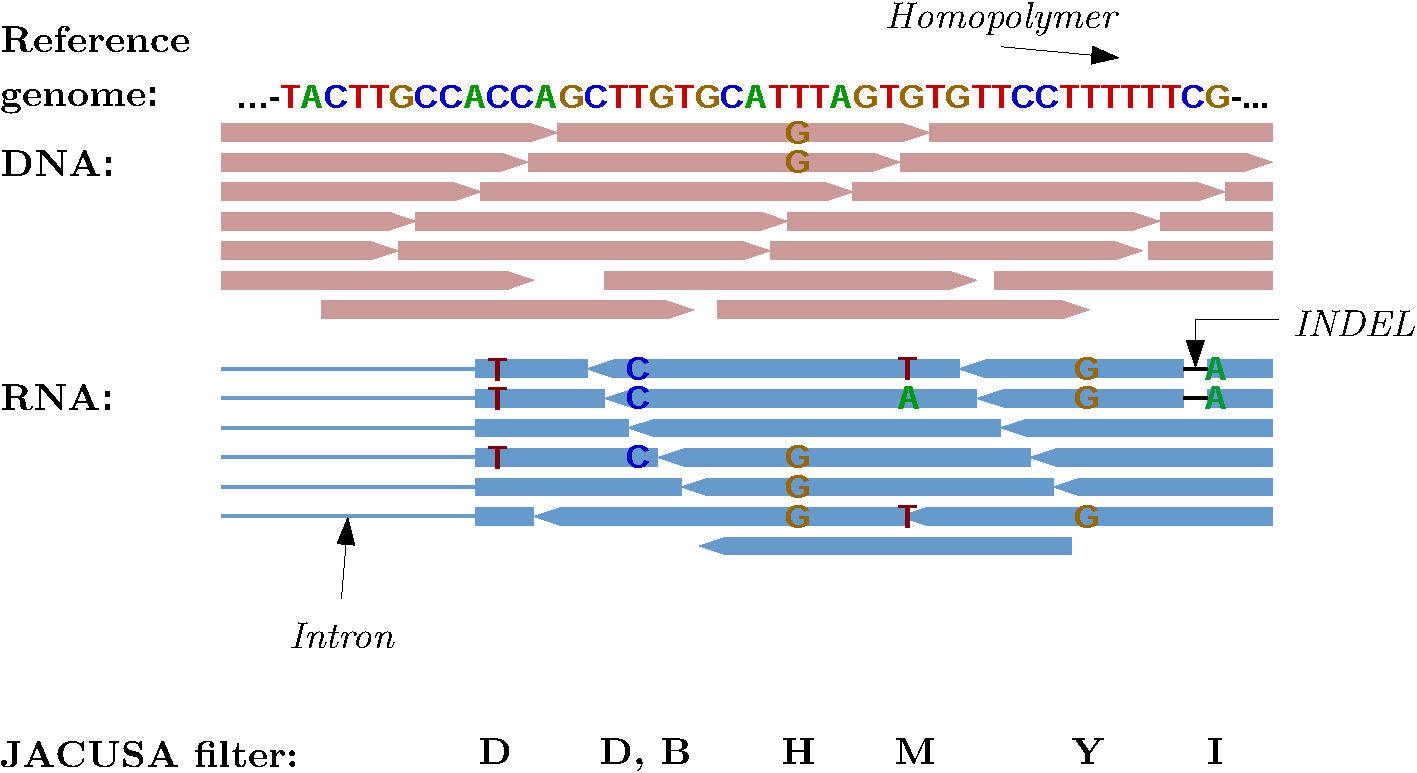
\includegraphics[width=\textwidth]{figures/jacusa_filter_cropped}
\end{figure}
\begin{tabular}{lp{.8\textwidth}}
\textbf{Value} & \textbf{Description of potential artefact} \\
\hline
D & Variant call in the vicinity of Read Start/End, Intron, and/or INDEL position \\
B & Variant call in the vicinity of Read Start/End \\
I & Variant call in the vicinity of INDEL position \\
S & Variant call in the vicinity of Splice Site \\
Y & Variant call in the vicinity of homopolymer \\
M & Max allowed alleles exceeded \\ 
H & ``Control'' sample contains non-homozygous pileup \\
\end{tabular}
\end{description}
%---------------------------------------------------------------------------------------------------
\section{Variant detection}
\subsection{Identification of RNA editing sites}
In order to identify RNA editing sites by comparing gDNA and \emph{stranded} RNA-Seq (single or paired end) use:
\begin{description} 
\item[first strand sequenced] ``-P1 UNSTRANDED -P2 RF-FIRSTSTRAND''
\item[second strand sequenced] ``-P2 UNSTRANDED -P2 FR-SECONDSTRAND''
\end{description}.
When your RNA-Seq is unstranded use: ``-P1 UNSTRANDED -P2 UNSTRANDED'' and infer the correct orientation from annnotation.

Use the following command line to identify RNA-DNA differences in BAM files that might give rise to RNA editing sites:
\begin{verbatim}
java -jar call-2 -r JACUSA.out -s -a H:1 gDNA.bam cDNA.bam
\end{verbatim}
Option ``-a H:1'' ensures that potential polymorphisms in gDNA will be eliminated as artefacts. The number $x \in \{1, 2\}$
determines which sample has to be homomorph - in this case: gDNA.bam.

Use the following command line to identify RNA-DNA differences:
\begin{verbatim}
java -jar call-2 -r JACUSA2.out -s cDNA1.bam cDNA2.bam
\end{verbatim}
WARNING: If you want to identify RNA-RNA differences make sure NOT to use the filter ``-a H:x''! Otherwise, potential valid variants will be filtered out. 
%---------------------------------------------------------------------------------------------------
\section{Reverse transcriptase arrest events}
%\todo[author=michael]{add text}
\section{Usage}
Calling JACUSA2 without any arguments will print the available tools which currently are:
\begin{verbatim}
java -jar JACUSA2.jar
  METHOD        DESCRIPTION
  call-1        Call variants - 1 condition
  call-2        Call variants - 2 conditions
  pileup        SAMtools like mpileup (2 conditions)
  rt-arrest     Reverse Transcription Arrest - 2 conditions
  lrt-arrest    Linkage arrest to base substitution - 2 conditions
Version: 		[...]
Libraries: 	
\end{verbatim}
%---------------------------------------------------------------------------------------------------
\subsection{call-1}
Single sample (call-1) allows to call variants against a reference. 
Internally, an \textit{in silico} sample is created from information that is provided by the ``MD'' field 
in BAM files.

The number of base columns depends on the number of BAM files. In basesIJ: $I$
corresponds to sample and $J$ to the respective replicate. Numbers indicate the base count of the
following base vector: $(A, C, G, T)$

Sites that have a $>$ alleles are considered candidate variant sites and for this sites a test-score will be computed.
\subsection{call-2}
%\todo[author=michael]{nicely combine call-1, call2}
%---------------------------------------------------------------------------------------------------
\subsection{pileup}
See ``Call variant - two samples'' for details.
\subsection{rt-arrest - 2 conditions}
In this method base call counts of arrest and read through reads are modelled by a Beta-Binomial distribution and 
differences between conditions are to be identified by means of a likelihood-ratio test. Subsequent approximiation 
with $\chi^2$ distribution to compute a pvalue.

Sites are considered candidate arrest sites, if in all BAM files there is at least one read through AND one  
read arrest event. Furthermore, coverage filter and minBASQ of Base Call apply that will affect the output. 
\subsection{lrt-arrest - 2 conditions}
%\todo[author=michael]{make fluent text}
lrt-arrest allows to link pileups to their arrest position. Output consists of read arrest and read through counts and 
a references to the associated arrest positions. There are cases, where currently an arrest position cannot be defined, 
e.g.: non properly paired reads.
Output consits of at least one line. Each separate arrest position adds an additional row is 
The first row contains the unstratified data or total, the ``arrest\_pos'' column is set to ``*''.
Any following sites with identical coordinates (contig, start, end, strand) will have a different 
arrest position reference in the ``arrest\_pos'' column. 

This method supports partial artefact filtering. Currently, filters only apply to the unstratified data --- 
sites with ``*'' in in ``arrest\_pos''. Furthermore, coverage filter and minBASQ of Base Call apply 
that will affect the output.
%---------------------------------------------------------------------------------------------------
% TODO options
\section{Description of command line options}
\subsection{Input / Output}
\subsubsection{Input BAM files}
% TODO BAM files
\subsubsection{Output file}
{\small
\begin{tabular}{@{}p{.25\textwidth}p{.5\textwidth}l@{}}
\multirow{5}{=}{-r RESULT-FILE} & \multirow{5}{=}{results are written to RESULT-FILE} & call-1 \\
 &  & call-2 \\
 &  & pileup \\
 &  & rt-arrest \\
 &  & lrt-arrest \\
\end{tabular}\\
}

%
\subsection{Filtering artefacts}
\subsubsection{Configure feature filter}
{\small
\begin{tabular}{@{}p{.25\textwidth}p{.5\textwidth}l@{}}
\multirow{5}{=}{-a FEATURE-FILTER} & \multirow{5}{=}{[...] Use -h to see extended help} & call-1 \\
 &  & call-2 \\
 &  & pileup \\
 &  & rt-arrest \\
 &  & lrt-arrest \\
\end{tabular}\\
}

\subsubsection{Output artefacts to separate file}
{\small
\begin{tabular}{@{}p{.25\textwidth}p{.5\textwidth}l@{}}
\multirow{5}{=}{-s FILTERED-FILE} & \multirow{5}{=}{Store feature-filtered results in another file (= RESULT-FILE.filtered if no argument) or (= FILTERED-FILE)} & call-1 \\
 &  & call-2 \\
 &  & pileup \\
 &  & rt-arrest \\
 &  & lrt-arrest \\
\end{tabular}\\
}

%
\subsection{Input BED file}
{\small
\begin{tabular}{@{}p{.25\textwidth}p{.5\textwidth}l@{}}
\multirow{5}{=}{-b BED} & \multirow{5}{=}{BED file to scan for variants} & call-1 \\
 &  & call-2 \\
 &  & pileup \\
 &  & rt-arrest \\
 &  & lrt-arrest \\
\end{tabular}\\
}

\subsection{Reference fasta file}
{\small
\begin{tabular}{@{}p{.25\textwidth}p{.5\textwidth}l@{}}
\multirow{5}{=}{-R REF-FASTA} & \multirow{5}{=}{use reference FASTA file (must be indexed)} & call-1 \\
 &  & call-2 \\
 &  & pileup \\
 &  & rt-arrest \\
 &  & lrt-arrest \\
\end{tabular}\\
}

%
\subsection{Library type}
{\small
\begin{tabular}{@{}p{.25\textwidth}p{.5\textwidth}l@{}}
\multirow{5}{=}{-P LIB-TYPE} & \multirow{3}{=}{Choose the library type for all conditions:
RF-FIRSTSTRAND	library - first strand sequenced
FR-SECONDSTRAND	library - second strand sequenced
UNSTRANDED	library
default: UNSTRANDED} & call-1 \\
 & & call-2 \\
 & & pileup \\
 & & rt-arrest \\
 & lrt-arrest \\
\end{tabular}\\
}

%
\subsection{Read base changes}
{\small
\begin{tabular}{@{}p{.25\textwidth}p{.5\textwidth}l@{}}
\multirow{4}{=}{-B READ-TAG} & \multirow{4}{=}{Tag reads by base substitution.
Count non-reference base substitution per read and stratify.
Requires stranded library type.
(Format for T to C mismatch: T2C; use ',' to separate substitutions)
Default: none} & call-1 \\
 &  & call-2 \\
 &  & pileup \\
 &  & rt-arrest \\
\end{tabular}\\
}

\subsection{Show deletion score}
{\small
\begin{tabular}{@{}p{.25\textwidth}p{.5\textwidth}l@{}}
\multirow{4}{=}{-D} & \multirow{4}{=}{Show deletion score} & call-1 \\
 &  & call-2 \\
 &  & pileup \\
 &  & rt-arrest \\
\end{tabular}\\
}

\subsection{General filtering}
\subsubsection{Filter by mapping quality}
{\small
\begin{tabular}{@{}p{.25\textwidth}p{.5\textwidth}l@{}}
\multirow{4}{=}{-m1 MIN-MAPQ1} & \multirow{4}{=}{filter positions with MAPQ < MIN-MAPQ1 for condition 1
default: 20} & call-2 \\
 &  & pileup \\
 &  & rt-arrest \\
 &  & lrt-arrest \\
\end{tabular}\\
}

\subsubsection{Filter by base call quality}
{\small
\begin{tabular}{@{}p{.25\textwidth}p{.5\textwidth}l@{}}
\multirow{4}{=}{-q1 MIN-BASQ1} & \multirow{4}{=}{filter positions with base quality < MIN-BASQ1 for condition 1
 default: 20} & call-2 \\
 &  & pileup \\
 &  & rt-arrest \\
 &  & lrt-arrest \\
\end{tabular}\\
}

\subsubsection{Filter by minimal coverage}
{\small
\begin{tabular}{@{}p{.25\textwidth}p{.5\textwidth}l@{}}
\multirow{4}{=}{-c1 MIN-COVERAGE1} & \multirow{4}{=}{filter positions with coverage < MIN-COVERAGE1 for condition 1
default: 5} & call-2 \\
 &  & pileup \\
 &  & rt-arrest \\
 &  & lrt-arrest \\
\end{tabular}\\
}

\subsubsection{Limit maximal depth}
{\small
\begin{tabular}{@{}p{.25\textwidth}p{.5\textwidth}l@{}}
\multirow{3}{=}{-d1 MAX-DEPTH1} & \multirow{3}{=}{max read depth for condition 1
default: -1} & call-2 \\
 &  & pileup \\
 &  & lrt-arrest \\
\end{tabular}\\
}

\subsection{Specific filtering}
\subsubsection{Filter by flag(s)}
% TODO escape latex letters {\small
\begin{tabular}{@{}p{.25\textwidth}p{.5\textwidth}l@{}}
\multirow{3}{=}{-f OUTPUT-FORMAT} & Choose output format: \protect\newline
<*> B: BED6-extended result format \protect\newline
< > V: VCF Output format. \protect\newline
Option -P will be ignored (VCF is unstranded)
 & call-1 \\
 & Choose output format: \protect\newline
<*> B: BED6-extended result format \protect\newline
< > V: VCF Output format. \protect\newline
Option -P will be ignored (VCF is unstranded)
 & call-2 \\
 & Choose output format: \protect\newline
<*> B: Default \protect\newline
< > M: samtools mpileup like format
 & pileup \\
\end{tabular}\\
}

\subsubsection{Retain by flag(s)}
{\small
\begin{tabular}{@{}p{.25\textwidth}p{.5\textwidth}l@{}}
\multirow{5}{=}{-F FLAG} & filter reads with flags FLAG
default: 0 & call-1 \\
 & \multirow{4}{=}{filter reads with flags FLAG for all conditions
default: 0} & call-2 \\
 & & pileup \\
 & & rt-arrest \\
 & & lrt-arrest \\
\end{tabular}\\
}

\subsubsection{Filter by number of hits}
{\small
\begin{tabular}{@{}p{.25\textwidth}p{.5\textwidth}l@{}}
\multirow{4}{=}{-filterNH\_1 NH} & \multirow{4}{=}{Max NH-VALUE for SAM tag NH for condition 1} & call-2 \\
 &  & pileup \\
 &  & rt-arrest \\
 &  & lrt-arrest \\
\end{tabular}\\
}

\subsubsection{Filter by number of mismatches}
{\small
\begin{tabular}{@{}p{.25\textwidth}p{.5\textwidth}l@{}}
\multirow{4}{=}{-filterNM\_1 NM} & \multirow{4}{=}{Max NM-VALUE for SAM tag NM for condition 1} & call-2 \\
 &  & pileup \\
 &  & rt-arrest \\
 &  & lrt-arrest \\
\end{tabular}\\
}

% 
\subsection{Thread related}
\subsubsection{Number of parallel threads}
{\small
\begin{tabular}{@{}p{.25\textwidth}p{.5\textwidth}l@{}}
\multirow{5}{=}{-p THREADS} & \multirow{5}{=}{use \# THREADS 
 default: 1} & call-1 \\
 &  & call-2 \\
 &  & pileup \\
 &  & rt-arrest \\
 &  & lrt-arrest \\
\end{tabular}\\
}

\subsubsection{Actual thread window size}
{\small
\begin{tabular}{@{}p{.25\textwidth}p{.5\textwidth}l@{}}
\multirow{5}{=}{-w WINDOW} & \multirow{4}{=}{size of the window used for caching. Make sure this is greater than the read size 
 default: 10000} & call-1 \\
 &  & call-2 \\
 &  & pileup \\
 & size of the window used for caching. Make sure this is greater than the read size 
 default: 10000 & rt-arrest \\
 & size of the window used for caching. Make sure this is greater than the read size 
 default: 5000 & lrt-arrest \\
\end{tabular}\\
}

\subsubsection{Reserved thread window size}
{\small
\begin{tabular}{@{}p{.25\textwidth}p{.5\textwidth}l@{}}
\multirow{5}{=}{-W THREAD-WINDOW} & \multirow{5}{=}{size of the window used per thread
default: 100000} & call-1 \\
 &  & call-2 \\
 &  & pileup \\
 &  & rt-arrest \\
 &  & lrt-arrest \\
\end{tabular}\\
}

%
\subsection{Test-statistic options}
{\small
\begin{tabular}{@{}p{.25\textwidth}p{.5\textwidth}l@{}}
\multirow{4}{=}{-T THRESHOLD} & \multirow{4}{=}{Filter positions based on test-statistic THRESHOLD
 default: DO NOT FILTER} & call-1 \\
 &  & call-2 \\
 &  & rt-arrest \\
 &  & lrt-arrest \\
\end{tabular}\\
}

{\small
\begin{tabular}{@{}p{.25\textwidth}p{.5\textwidth}l@{}}
\multirow{4}{=}{-u MODE} & \multirow{4}{=}{[...] Use -h to see extended help} & call-1 \\
 &  & call-2 \\
 &  & rt-arrest \\
 &  & lrt-arrest \\
\end{tabular}\\
}

\subsection{Filtering by Test-statistic threshold}
% TODO remove
%\clioption{-T <THRESHOLD>}{Filter positions based on test-statistic THRESHOLD\newline default: DO 
%NOT FILTER}{\callone \calltwo \rtarrest \lrtarrest}
\subsection{Misc}
{\small
\begin{tabular}{@{}p{.25\textwidth}p{.5\textwidth}l@{}}
\multirow{5}{=}{-h} & \multirow{5}{=}{Print extended usage information} & call-1 \\
 &  & call-2 \\
 &  & pileup \\
 &  & rt-arrest \\
 &  & lrt-arrest \\
\end{tabular}\\
}

{\small
\begin{tabular}{@{}p{.25\textwidth}p{.5\textwidth}l@{}}
\multirow{5}{=}{-x} & \multirow{5}{=}{turn on Debug modus} & call-1 \\
 &  & call-2 \\
 &  & pileup \\
 &  & rt-arrest \\
 &  & lrt-arrest \\
\end{tabular}\\
}

%---------------------------------------------------------------------------------------------------
\section{Used libraries}
\begin{tabular}{lrl}
\bf{Libray} & \bf{Version} & \bf{Source} \\
\hline
htsjdk & 2.12.0 & \url{https://github.com/samtools/htsjdk} \\
Apache commons-cli & 1.4 & \url{https://commons.apache.org/proper/commons-cli} \\
Apache commons-math3 & 3.6.1 & \url{http://commons.apache.org/proper/commons-math}
\end{tabular}
%---------------------------------------------------------------------------------------------------
\bibliographystyle{apalike}
\bibliography{manual}
%---------------------------------------------------------------------------------------------------
\end{document}
%---------------------------------------------------------------------------------------------------